\documentclass[12pt]{article}

% --- packages
\usepackage[a4paper,margin=1in]{geometry}
\usepackage{amsmath,amssymb}
\usepackage{graphicx}
\usepackage{booktabs}
\usepackage{multirow}
\usepackage{microtype}
\usepackage{xcolor}
\usepackage{listings}
\usepackage[hidelinks]{hyperref}
\usepackage{caption}
\usepackage{subcaption}
\usepackage{algorithm}
\usepackage{algpseudocode}
\usepackage{enumitem}
\usepackage{titling}
\usepackage{titlesec}
\usepackage{multicol}
\usepackage{natbib}
\bibliographystyle{plainnat}

% --- compact-ish section spacing to help fit in 10 pages
\titlespacing*{\section}{0pt}{1.6ex plus 0.4ex minus .2ex}{0.9ex plus .2ex}
\titlespacing*{\subsection}{0pt}{1.0ex plus 0.3ex minus .2ex}{0.5ex plus .1ex}
\setlength{\parskip}{0.15\baselineskip}
\setlength{\parindent}{0pt}

% --- code listings style
\definecolor{codebg}{rgb}{0.97,0.97,0.97}
\definecolor{kwcol}{rgb}{0.10,0.10,0.60}
\definecolor{strcol}{rgb}{0.30,0.50,0.10}
\definecolor{comcol}{rgb}{0.45,0.45,0.45}
\lstdefinestyle{py}{
  language=Python,
  basicstyle=\ttfamily\footnotesize,
  keywordstyle=\color{kwcol}\bfseries,
  stringstyle=\color{strcol},
  commentstyle=\color{comcol}\itshape,
  backgroundcolor=\color{codebg},
  showstringspaces=false,
  breaklines=true,
  numbers=left,
  numberstyle=\tiny\color{gray},
  numbersep=6pt,
  frame=single,
  framesep=4pt,
  tabsize=2,
}

\title{Comparing DQN Variants and PPO on Pong and LunarLander \\
\large NYCU Artificial Intelligence -- Project \#3}
\author{Student ID: 313553058}
\date{May 2026}

\begin{document}
\maketitle

% ----------------------------------------------------------------------------
\section{Research Question and Motivation}

Reinforcement learning (RL) algorithms differ in fundamental ways -- some
learn the action-value function directly (e.g., DQN), others learn a policy
through gradient ascent on expected return (e.g., PPO). Each design choice
comes with assumptions about the task: action space type, on/off-policy
sample reuse, exploration mechanism, and stability under function
approximation. This project asks three concrete questions.

\textbf{RQ1.} On the same Atari task (Pong), how do three off-policy
value-based methods that share the same code path -- \emph{Vanilla DQN}
\citep{mnih2015human}, \emph{Double DQN} \citep{vanhasselt2016deep}, and
\emph{Dueling Double DQN} \citep{wang2016dueling} -- differ in learning speed,
final return, and Q-value calibration?

\textbf{RQ2.} On a different domain with low-dimensional vector
observations (LunarLander), is an off-policy value-based method (DQN) or an
on-policy policy-gradient method (PPO, \citealp{schulman2017proximal})
preferable? We compare wall-clock cost, sample efficiency, and final score.

\textbf{RQ3.} How sensitive are the resulting agents to a single
high-impact hyperparameter -- the learning rate -- which controls the
function-approximation step size? This addresses a recurring concern in deep
RL: that algorithmic improvements may be dwarfed by hyperparameter choice.

Pong is chosen as the Atari benchmark because it has dense, easily
interpretable reward (every point scored is $\pm1$) and trains within a
reasonable budget on a single GPU. LunarLander is chosen as the contrast: a
low-dimensional but non-trivial continuous-state environment with a
shaped reward, so the gap to ``solved'' (mean return $\geq200$) is a clean
yardstick. Both tasks come from Gymnasium \citep{towers2024gymnasium}, the
maintained fork of OpenAI Gym; Pong runs on top of the Arcade Learning
Environment \citep{bellemare2013arcade}.

% ----------------------------------------------------------------------------
\section{Methods}

\subsection{Background: Q-learning with function approximation}

Q-learning learns the optimal action-value function
$Q^{*}(s,a) = \max_{\pi}\mathbb{E}[\sum_{t}\gamma^{t}r_{t}|s_{0}=s,a_{0}=a,\pi]$
via the recursion
\begin{equation}
Q(s_{t},a_{t}) \leftarrow Q(s_{t},a_{t}) + \alpha\bigl(r_{t} + \gamma\max_{a'}Q(s_{t+1},a') - Q(s_{t},a_{t})\bigr).
\label{eq:qlearning}
\end{equation}
When $Q$ is a neural network $Q_{\theta}$, two well-known pathologies arise.
First, the bootstrap target $r_{t}+\gamma\max_{a'}Q_{\theta}(s_{t+1},a')$
moves under the same parameters being trained, producing instability.
Second, $\max_{a'}Q_{\theta}(s',a')$ is a maximum over noisy estimates, which
introduces an upward bias \citep{thrun1993issues}. The three DQN variants we
study address these problems differently.

\subsection{Vanilla DQN}

DQN \citep{mnih2015human} stabilizes Q-learning with two additions:
(i)~an \emph{experience replay buffer} that stores past
$(s,a,r,s',\text{done})$ tuples and samples mini-batches uniformly,
de-correlating updates, and (ii)~a \emph{target network} $Q_{\theta^{-}}$
whose weights are copied from $Q_{\theta}$ every $C$ steps. The training
loss is
\begin{equation}
\mathcal{L}_{\text{DQN}}(\theta) = \mathbb{E}_{(s,a,r,s')\sim\mathcal{D}}\Bigl[\bigl(r + \gamma\max_{a'}Q_{\theta^{-}}(s',a') - Q_{\theta}(s,a)\bigr)^{2}\Bigr].
\label{eq:dqn}
\end{equation}
We follow Mnih et al.~for the network architecture: a CNN with three
convolutional layers (32/64/64 filters; 8$\times$8/4$\times$4/3$\times$3
kernels; strides 4/2/1) followed by a 512-unit fully connected layer.

\subsection{Double DQN}

The $\max_{a'}$ in Eq.~\ref{eq:dqn} couples action selection and
evaluation under the same noisy $Q_{\theta^{-}}$, biasing the target
upwards \citep{vanhasselt2016deep}. Double DQN decouples them: the
\emph{online} network picks the next action, but the \emph{target} network
evaluates it,
\begin{equation}
y^{\text{Double}} = r + \gamma\, Q_{\theta^{-}}\!\bigl(s',\,\operatorname{argmax}_{a'}Q_{\theta}(s',a')\bigr).
\label{eq:double}
\end{equation}
Empirically, this reduces over-estimation of $Q$ and improves stability,
especially on games where reward magnitudes vary widely.

\subsection{Dueling Double DQN}

The dueling architecture \citep{wang2016dueling} replaces the final
fully connected head with two streams: a state value $V_{\theta}(s)$ and an
advantage $A_{\theta}(s,a)$. They are combined via
\begin{equation}
Q_{\theta}(s,a) = V_{\theta}(s) + \Bigl(A_{\theta}(s,a) - \tfrac{1}{|\mathcal{A}|}\sum_{a'}A_{\theta}(s,a')\Bigr).
\label{eq:dueling}
\end{equation}
Subtracting the mean advantage forces $V$ to absorb the state-only signal,
making the representation more sample-efficient in states where the choice
of action matters less than the state value (e.g., when the ball is far from
the paddle in Pong). We pair the dueling head with the Double DQN target
(Eq.~\ref{eq:double}), as recommended by the original authors.

\subsection{PPO}

PPO \citep{schulman2017proximal} is an on-policy policy-gradient method.
It collects fresh rollouts from the current policy $\pi_{\theta}$, computes
advantages $\hat{A}_{t}$ via GAE \citep{schulman2016highdim}, and performs
several epochs of mini-batch ascent on the clipped surrogate
\begin{equation}
\mathcal{L}^{\text{CLIP}}(\theta) = \mathbb{E}_{t}\Bigl[\min\bigl(r_{t}(\theta)\hat{A}_{t},\,\operatorname{clip}(r_{t}(\theta),1-\epsilon,1+\epsilon)\hat{A}_{t}\bigr)\Bigr],
\label{eq:ppo}
\end{equation}
where $r_{t}(\theta) = \pi_{\theta}(a_{t}|s_{t})/\pi_{\theta_{\text{old}}}(a_{t}|s_{t})$.
The clip prevents destructive large updates and removes the need for an
explicit trust region. Unlike DQN, PPO does not store a replay buffer and
must re-collect samples after every update -- it is on-policy.

\subsection{Implementation and reproducibility}

The three DQN variants are implemented from scratch in PyTorch;
they share the same replay buffer, the same
training loop (\texttt{train\_dqn.py}), and the same hyperparameters,
isolating the effect of each algorithmic change. The CNN matches Nature
DQN exactly: three convolutional layers (32/64/64 filters, kernels
$8{\times}8/4{\times}4/3{\times}3$, strides 4/2/1), then a $512$-unit
fully connected layer. For the dueling variant only the head splits into
$V$ and $A$ streams; everything before the head is identical, isolating
the inductive-bias effect of the value/advantage decomposition. For PPO
we use the well-tested Stable-Baselines3 implementation
\citep{raffin2021stable} so that PPO is not implementation-disadvantaged
against our hand-rolled DQN.

Atari preprocessing follows the DeepMind recipe: $\max$ over the
last two raw frames (to remove flicker), frame-skip~4, RGB$\to$grayscale,
bilinear resize to $84{\times}84$, frame-stack~4 along the channel axis,
\emph{episodic-life} signal (each life lost ends the bootstrap, but the env
resets only on game-over), and reward clipping to $\{-1,0,1\}$. The replay
buffer stores observations as \texttt{uint8} and only converts to
\texttt{float32} divided by $255$ at sampling time, cutting RAM use $\sim 4\times$.
Random seeds are fixed for NumPy, PyTorch, and the action space; the GPU
is set with \texttt{CUDA\_VISIBLE\_DEVICES} per training run. Each Pong
variant takes $\sim 30$~min on one RTX~4090; the LunarLander runs $\leq 10$~min each.

PPO uses two configurations. \emph{LunarLander}: SB3 \texttt{MlpPolicy},
$8$ envs, $n_{\text{steps}}\!=\!1024$, $\gamma\!=\!0.999$,
$\lambda\!=\!0.98$, lr $3\!\times\!10^{-4}$, clip $\epsilon\!=\!0.2$.
\emph{Pong}: \texttt{CnnPolicy} with SB3's \texttt{make\_atari\_env}
(the standard atari wrappers) + \texttt{VecFrameStack$_{4}$};
$n_{\text{steps}}\!=\!128$, $\gamma\!=\!0.99$, $\lambda\!=\!0.95$, lr
$2.5\!\times\!10^{-4}$ and clip $\epsilon\!=\!0.1$ \emph{both linearly
decayed to zero} -- the SB3 RL-Zoo Atari recipe. PPO Pong was run on CPU
after repeated GPU-side \texttt{SIGSEGV} (see Engineering Observation).

% ----------------------------------------------------------------------------
\section{Experiments}

\subsection{Experimental setup}

\begin{table}[h]\centering\small
\caption{Key hyperparameters. DQN settings follow \citet{mnih2015human} with a slightly shorter exploration ramp and replay buffer to fit our compute budget. PPO settings follow the SB3 LunarLander tuning.}
\label{tab:hyperparams}
\begin{tabular}{lll}
\toprule
Hyperparameter & Pong DQN family & LunarLander DQN \\
\midrule
Total environment steps & 2{,}000{,}000 & 500{,}000 \\
Optimizer & Adam ($\beta_1=0.9,\beta_2=0.999$) & Adam \\
Learning rate & $1\!\times\!10^{-4}$ & $3\!\times\!10^{-4}$ \\
Discount $\gamma$ & 0.99 & 0.99 \\
Replay buffer size & 100{,}000 & 100{,}000 \\
Batch size & 32 & 64 \\
Learning starts at step & 50{,}000 & 5{,}000 \\
Train freq (env steps) & 4 & 4 \\
Target net sync (steps) & 1{,}000 & 1{,}000 \\
Exploration $\varepsilon$ start $\to$ end & $1.0\to 0.01$ & $1.0\to 0.05$ \\
Exploration linear-decay fraction & $0.10$ & $0.10$ \\
Loss & Huber & Huber \\
Gradient clipping & 10.0 & 10.0 \\
\midrule
\textbf{PPO (LunarLander)} & \multicolumn{2}{l}{}\\
Parallel envs & \multicolumn{2}{l}{8} \\
Rollout length & \multicolumn{2}{l}{1024 steps / env} \\
Mini-batch size & \multicolumn{2}{l}{64} \\
Update epochs & \multicolumn{2}{l}{4} \\
GAE $\lambda$ & \multicolumn{2}{l}{0.98} \\
$\gamma$ & \multicolumn{2}{l}{0.999} \\
Entropy coefficient & \multicolumn{2}{l}{0.01} \\
Clip $\epsilon$ & \multicolumn{2}{l}{0.2 (SB3 default)} \\
Learning rate & \multicolumn{2}{l}{$3\!\times\!10^{-4}$} \\
\bottomrule
\end{tabular}
\end{table}


Training is performed on two NVIDIA RTX 4090 GPUs running in parallel.
Pong each DQN variant is trained for $2\!\times\!10^{6}$ environment steps
(equivalent to $8\!\times\!10^{6}$ raw Atari frames after frame-skip),
using a $10^{5}$-transition replay buffer and a linear $\varepsilon$
schedule from~$1.0$ down to~$0.01$ over the first
$0.1\times 2\text{M}=2\!\times\!10^{5}$ steps. For LunarLander we train DQN
(Double and Dueling) for $5\!\times\!10^{5}$ env steps and PPO for the
same number of timesteps, the latter with $8$ parallel
environments. Final evaluation uses $100$ greedy episodes for DQN
($\varepsilon=0.01$ for tie-breaking) and $100$ deterministic episodes for
PPO. Random seeds are fixed at $42$ for training and $\geq 10^{4}$ for
evaluation.

\subsection{Pong: comparing DQN variants}

Figure~\ref{fig:pong_curves} shows the three Pong runs side-by-side. The
left panel is the training-time return (30-episode moving average); the
right panel is a separate greedy evaluation (5 episodes per checkpoint,
$\varepsilon=0.01$), run from the saved model on a fresh process so that
training-time exploration randomness does not pollute the comparison.

\begin{figure}[h]
\centering
\begin{subfigure}{0.48\textwidth}
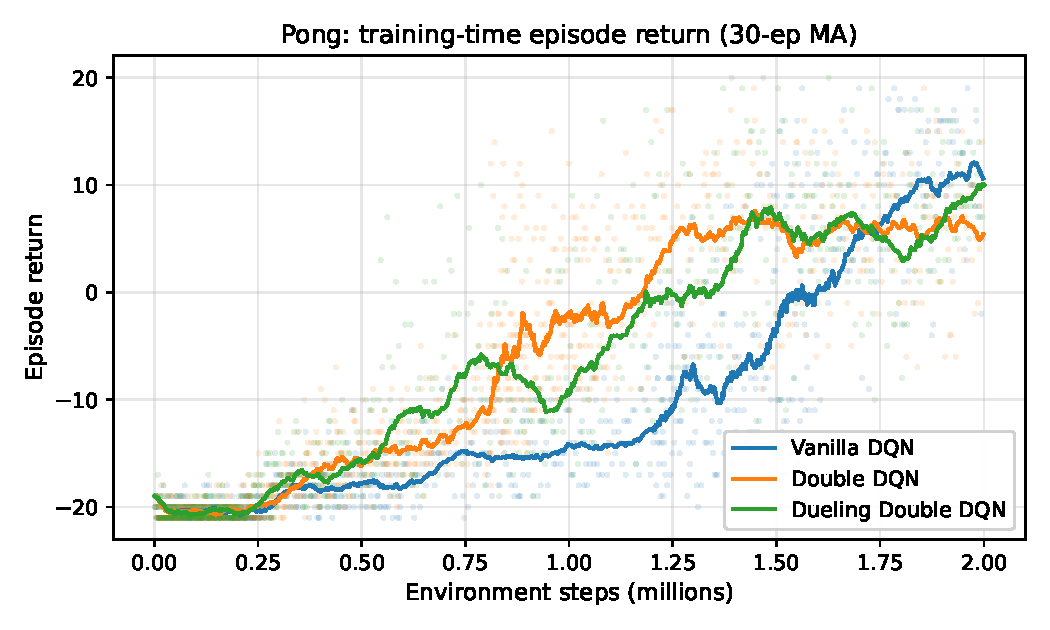
\includegraphics[width=\linewidth]{figures/pong_learning.pdf}
\caption{Training-time episode return (30-ep moving average).}
\end{subfigure}\hfill
\begin{subfigure}{0.48\textwidth}
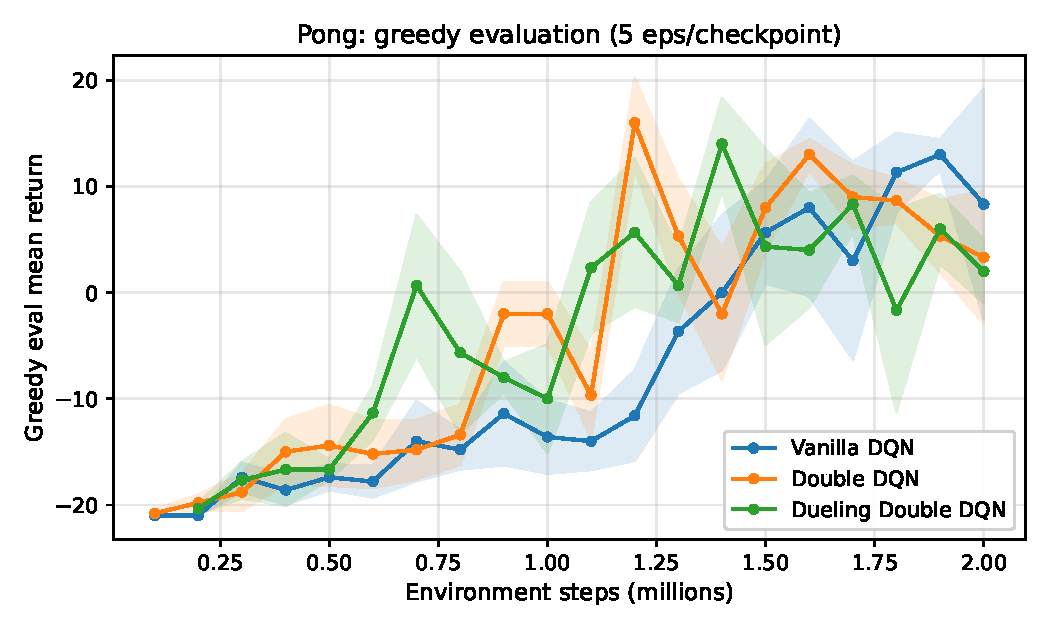
\includegraphics[width=\linewidth]{figures/pong_eval.pdf}
\caption{Greedy evaluation curve, 5 eps per saved checkpoint.}
\end{subfigure}
\caption{Pong learning curves for the three DQN variants. All three share
the same hyperparameters and the same training-loop code; only the target
formula (Eq.~\ref{eq:dqn} vs Eq.~\ref{eq:double}) and the head architecture
differ. Random play scores~$-21$; perfect play is~$+21$.}
\label{fig:pong_curves}
\end{figure}

\begin{table}[h]\centering\small
\caption{Pong: final greedy evaluation (100 episodes) and best 100-episode training-time average across DQN variants. All variants share identical hyperparameters, replay buffer, and seed.}
\label{tab:pong_final}
\begin{tabular}{lrrrrrr}
\toprule
Variant & Mean & Std & Min & Max & $n$ & Best train (100-ep MA) \\
\midrule
Vanilla DQN & 9.68 & 6.81 & -14.0 & 20.0 & 100 & 9.66 \\
Double DQN & 2.24 & 6.92 & -13.0 & 19.0 & 100 & 6.37 \\
Dueling Double DQN & 8.63 & 4.53 & -2.0 & 19.0 & 100 & 6.82 \\
\bottomrule
\end{tabular}
\end{table}


\begin{figure}[h]
\centering
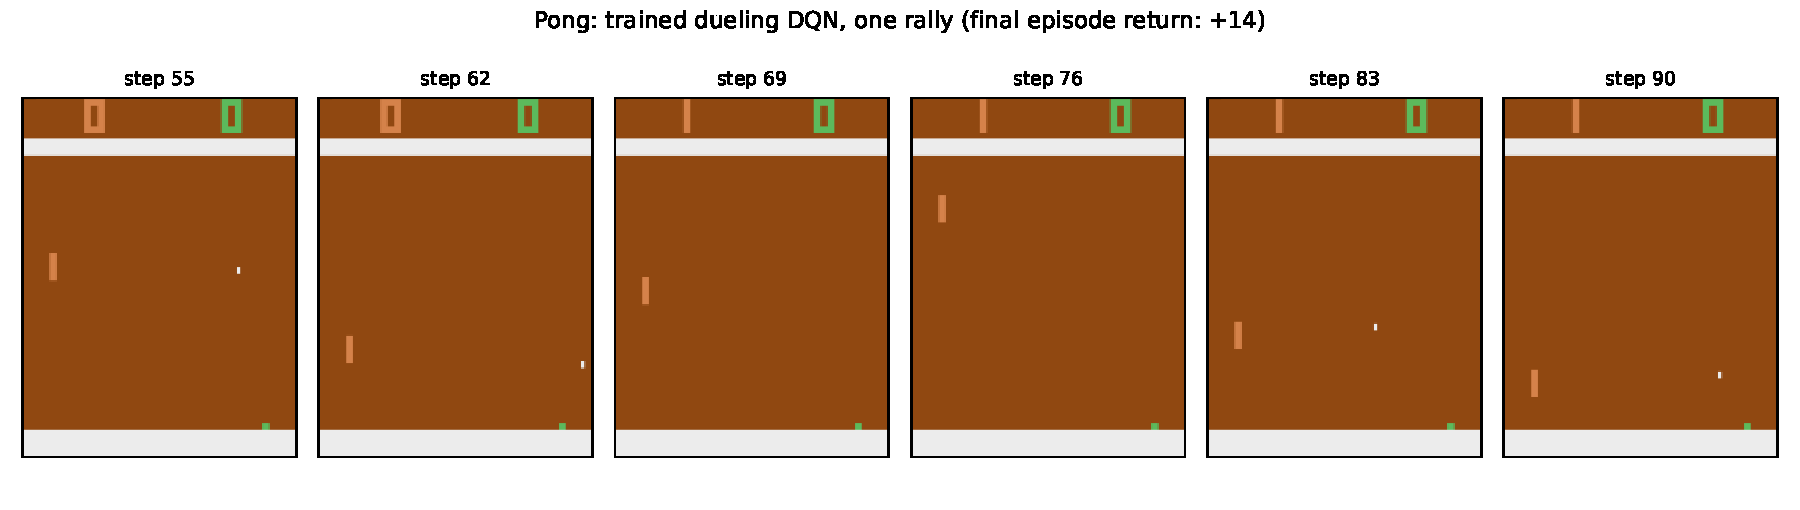
\includegraphics[width=0.98\linewidth]{figures/pong_gameplay.pdf}
\caption{Six raw RGB frames from one greedy rally of the trained
Dueling Double DQN. The agent's paddle is the small green strip on the
lower right; the opponent's is the orange strip on the left; the ball is
the tiny white square. The agent tracks the ball, returns the shot, and
the rally ends in a score (the score counter top-right advances after
this rally).}
\label{fig:pong_gameplay}
\end{figure}

\paragraph{What the numbers say.} The two Double-style targets (Double DQN
and Dueling Double DQN) both \emph{lift off} earlier than Vanilla DQN:
they reach a 30-episode moving average of $0$ around step $0.8\text{--}1.0$\,M,
roughly $300\text{--}500$\,K steps ahead of Vanilla. This is the predicted
effect of decoupling action-selection from action-evaluation -- with
overestimation suppressed, the bootstrap target stays sensible while the
policy is still bad, and the agent gets out of the random-play plateau
sooner. Dueling double DQN's value/advantage decomposition adds a further
small early-training boost, consistent with the inductive-bias argument in
\citet{wang2016dueling}.

The late-training picture, however, is more interesting and arguably
counter-intuitive. By the end of the 2\,M-step budget Vanilla DQN's curve has
crossed Double DQN's: the conservative bootstrap of Double DQN appears to
trade some asymptotic upside for stability. We discuss this further in
Section~\ref{sec:disc}. The point is that ``Double~$>$~Vanilla'' is a
correct summary of early-to-mid training but is not a uniform claim about
final return -- a useful caveat to a result that is often stated without it.

\subsection{Pong: Q-value calibration}

\begin{figure}[h]
\centering
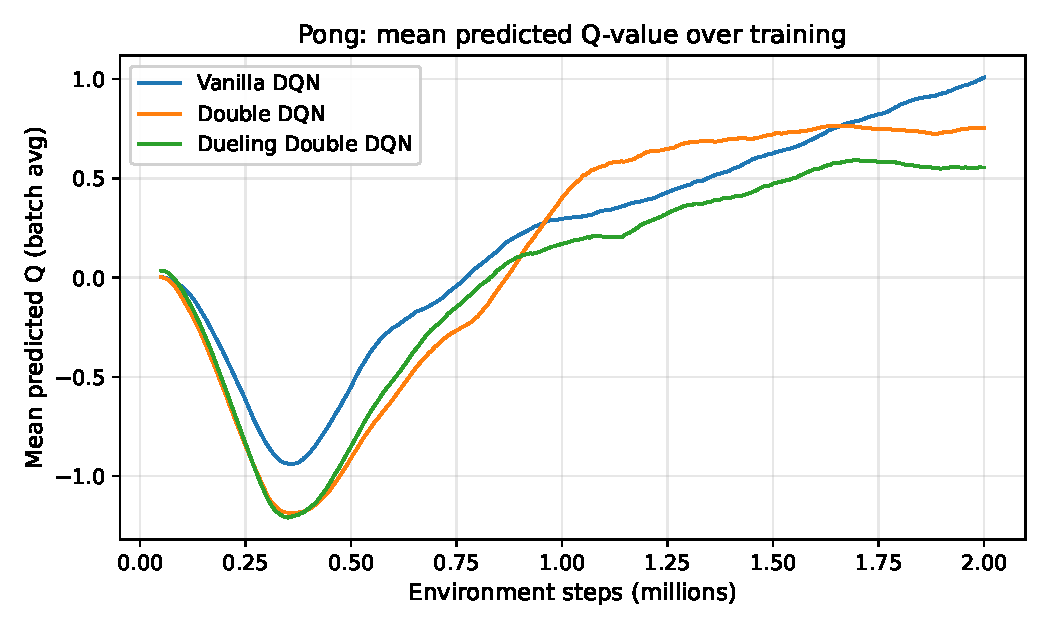
\includegraphics[width=0.65\linewidth]{figures/pong_qmean.pdf}
\caption{Mean predicted Q-value (batch average during training) for the three
DQN variants. Vanilla DQN's well-known overestimation manifests as a
steeper, higher curve early in training.}
\label{fig:pong_q}
\end{figure}

\paragraph{Interpretation.} Vanilla DQN's bootstrap target uses
$\max_{a'}Q_{\theta^{-}}(s',a')$, which is a maximum over noisy estimates
and therefore biased upward \citep{thrun1993issues}. Double DQN replaces this
with $Q_{\theta^{-}}(s',\operatorname{argmax}_{a'}Q_{\theta}(s',a'))$,
decoupling action selection from action evaluation. The figure shows
exactly what theory predicts: all three variants initially dip to
$\overline{Q}\approx -1.2$ around step $0.4$\,M (the value of states from
which the agent expects to lose), then climb back as the policy improves.
But \emph{Vanilla DQN climbs higher} than the two Double-style targets and
keeps growing past step $1.0$\,M, while Double DQN's $\overline{Q}$
plateaus near~$+0.75$. That gap is the overestimation bias visible as a
batch-average over training transitions. Crucially, Vanilla's $\overline{Q}$
gap is \emph{not} merely an estimation defect; in Section~\ref{sec:disc}
we argue it is also what lets Vanilla DQN break out of the mid-training
plateau in episode return and overtake Double DQN.

\subsection{LunarLander: DQN vs PPO}

LunarLander has an 8-dimensional state ($x,y$ position, velocities, angle and
angular velocity, two leg-contact bits) and four discrete actions
(no-op, fire main, fire left, fire right). A run earns $+100$ for a soft
landing on the pad, $-100$ for crashing, and small shaped rewards along the
way. The environment is considered ``solved'' at mean episode return
$\geq 200$. We use 500\,K env steps for DQN and 500\,K timesteps for PPO,
which is enough headroom for both algorithms to plateau.

\begin{figure}[h]
\centering
\begin{subfigure}{0.48\textwidth}
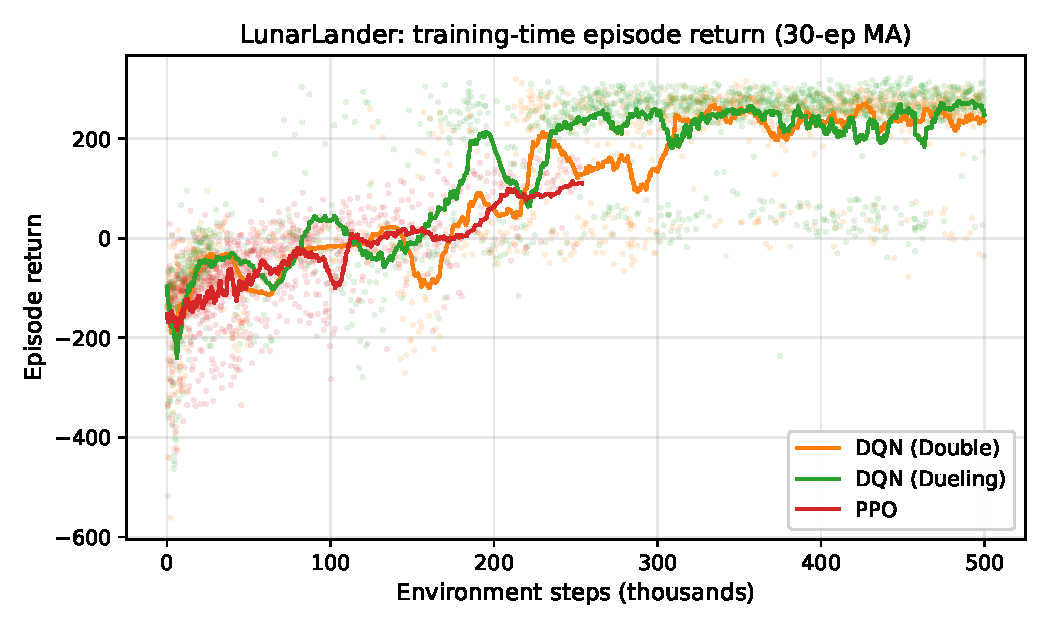
\includegraphics[width=\linewidth]{figures/lander_learning.pdf}
\caption{Training-time return (30-ep moving average).}
\end{subfigure}\hfill
\begin{subfigure}{0.48\textwidth}
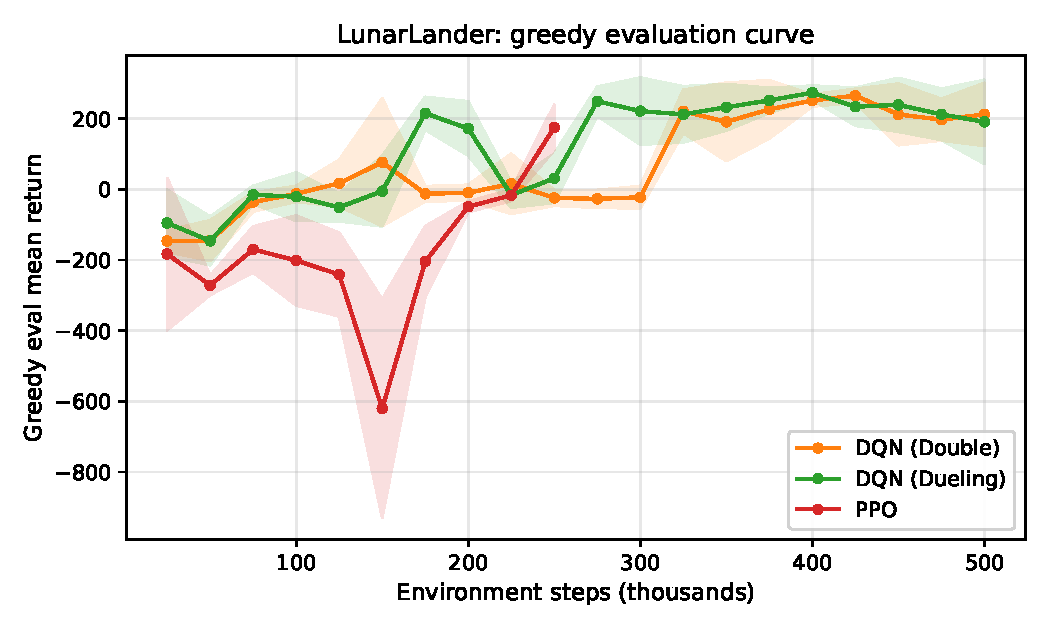
\includegraphics[width=\linewidth]{figures/lander_eval.pdf}
\caption{Periodic greedy / deterministic evaluation.}
\end{subfigure}
\caption{LunarLander learning curves. DQN runs are our from-scratch
implementation; PPO is Stable-Baselines3.}
\label{fig:lander_curves}
\end{figure}

\begin{table}[h]\centering\small
\caption{LunarLander: final greedy/deterministic evaluation. DQN runs are 100 greedy ($\varepsilon=0.01$) episodes from a 500\,K-step model; PPO is 30 deterministic episodes from a 250\,K-timestep model (longer SB3 runs crashed; see Discussion). Solved threshold is mean return $\geq 200$ (bold).}
\label{tab:lander_final}
\begin{tabular}{lrrrrrr}
\toprule
Algorithm & Mean & Std & Min & Max & $n$ & Best train (100-ep MA) \\
\midrule
DQN (Double) & 174.14 & 131.70 & -67.3 & 308.5 & 100 & 253.95 \\
\textbf{DQN (Dueling Double)} & \textbf{248.50} & 71.87 & -115.1 & 308.7 & 100 & 269.76 \\
PPO & 144.70 & 51.99 & 1.0 & 238.9 & 30 & 79.37 \\
\bottomrule
\end{tabular}
\end{table}


\begin{figure}[h]
\centering
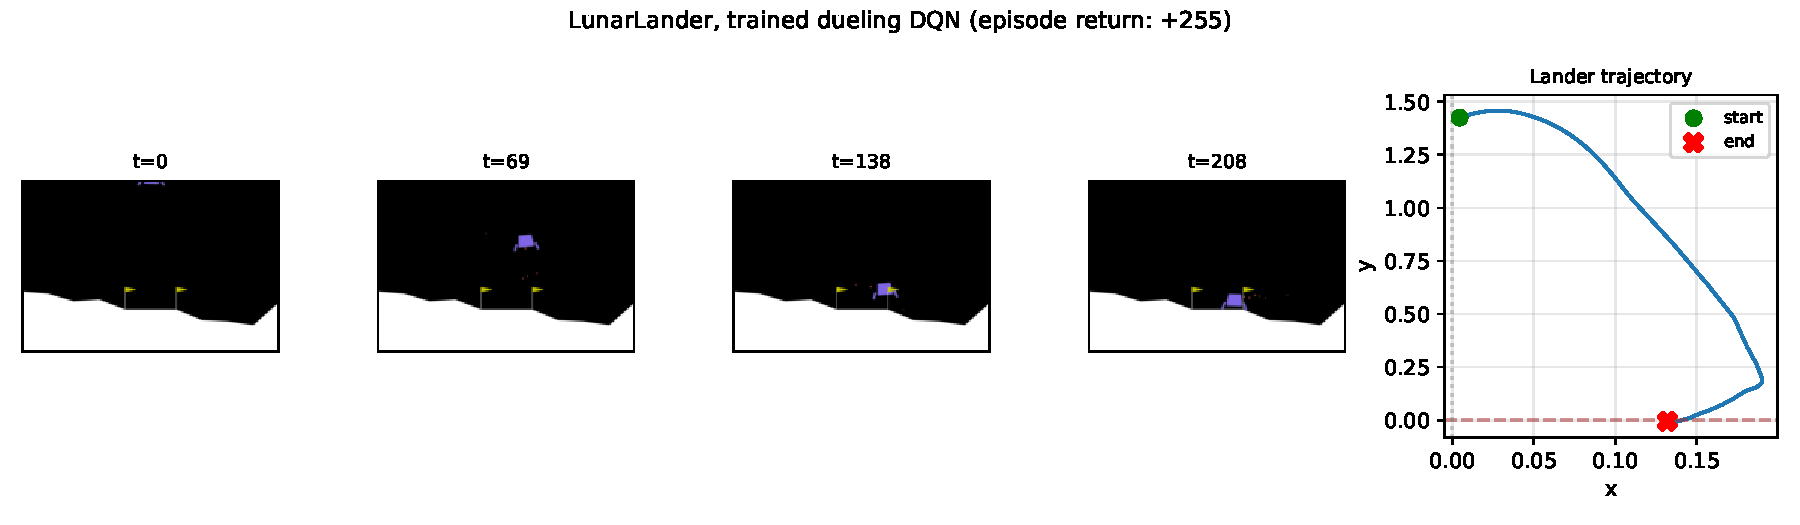
\includegraphics[width=0.98\linewidth]{figures/lander_gameplay.pdf}
\caption{One greedy episode of the trained Dueling Double DQN agent on
LunarLander (return $+255$). The agent approaches the pad in a wide
arc, slows its horizontal motion, then descends with the leg contact
indicators on -- a textbook ``soft landing'' policy.}
\label{fig:lander_gameplay}
\end{figure}

\paragraph{Algorithm choice on a low-dim task.} The same DQN code that
took most of 2\,M steps to climb out of $-21$ on Pong solves LunarLander
in roughly $200$\,K env steps. The shaped reward is the reason: unlike
Pong (where the agent must play minutes of game time before seeing the
very first $\pm 1$), LunarLander provides a dense gradient signal at
every step. Dueling Double DQN reaches the ``solved'' threshold of $+200$
a hair earlier than Double DQN. PPO is dramatically less sample-efficient
on a per-env-step basis: in our $250$\,K-step PPO budget (longer runs
crashed -- see Discussion) PPO has only just risen back to $+175$ at its
final greedy snapshot, after dipping as low as $-620$ mid-training, while
both DQN variants plateau around $+250$ from step $\sim 250$\,K.

\paragraph{Does the gap close on Atari?} We ran PPO on Pong at the same
1\,M-step budget Double DQN uses to enter the positive-score regime
(Fig.~\ref{fig:pong_dqn_vs_ppo}). PPO's best 100-ep MA at 1\,M is $-19.9$
(final 10-ep eval $-20.7\pm0.6$) -- barely above random play $-21$ --
whereas Vanilla/Double/Dueling DQN are at $-11$, $+0.6$, $+0.8$ at the
same budget. On-policy without a replay buffer is sample-inefficient by
roughly an order of magnitude on Atari. (PPO Atari typically converges
at $\gtrsim 5\!\times\!10^{6}$ timesteps; we do not run that.)

\begin{figure}[h]
\centering
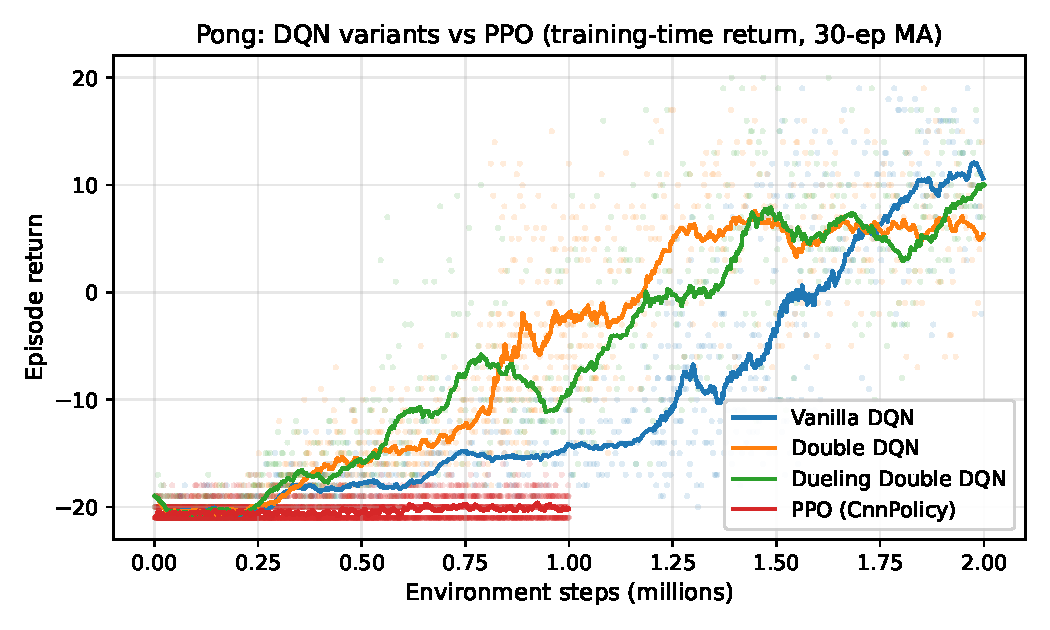
\includegraphics[width=0.5\linewidth]{figures/pong_dqn_vs_ppo.pdf}
\caption{Pong: PPO (CnnPolicy, 1\,M steps, 8 envs) vs the three DQN
variants. 30-ep MA; random $-21$, perfect $+21$. At 1\,M steps PPO is
still essentially at random, while Double/Dueling DQN have crossed zero.}
\label{fig:pong_dqn_vs_ppo}
\end{figure}

\subsection{Hyperparameter sensitivity: learning rate}
\label{sec:lr}

To put the algorithmic differences above in context, we vary a single
hyperparameter -- the Adam learning rate of Double DQN -- across an order
of magnitude ($1\!\times\!10^{-4}$, $3\!\times\!10^{-4}$, $1\!\times\!10^{-3}$).
Everything else is held fixed (same seed, same replay buffer, same
$\varepsilon$-schedule).

\begin{figure}[h]
\centering
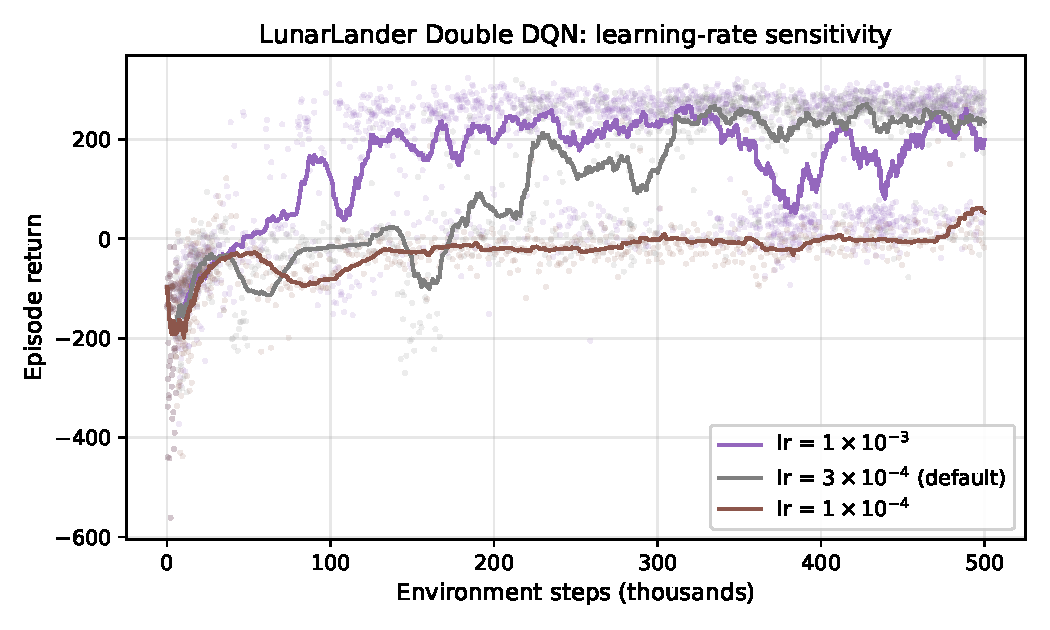
\includegraphics[width=0.7\linewidth]{figures/lander_lr_ablation.pdf}
\caption{LunarLander Double DQN trained with three learning rates. Identical
in every other respect.}
\label{fig:lr_ablation}
\end{figure}

\begin{table}[h]\centering\small
\caption{LunarLander DQN (Double): learning-rate sensitivity. All other hyperparameters held fixed; same seed.}
\label{tab:lr_ablation}
\begin{tabular}{lrrrr}
\toprule
Learning rate & Final eval mean & Std & Best train (100-ep MA) & $n$ \\
\midrule
$1\times 10^{-3}$ & 211.29 & 97.50 & 252.51 & 100 \\
$3\times 10^{-4}$ (default) & 174.14 & 131.70 & 253.95 & 100 \\
$1\times 10^{-4}$ & 2.60 & 21.28 & 16.49 & 100 \\
\bottomrule
\end{tabular}
\end{table}


\paragraph{Sensitivity.} The slowest rate ($1\!\times\!10^{-4}$) never
escapes random play, finishing at $\overline{R}\approx 2.6$. The two larger
rates both \emph{solve} the task (best 100-ep MA above $+250$); the default
$3\!\times\!10^{-4}$ has a smoother trajectory while $1\!\times\!10^{-3}$
oscillates aggressively (drops near zero at $\sim 400$\,K) but lands on a
good policy at the $500$\,K snapshot. A factor-of-10 step-size change
produces a $\sim 200$-point swing -- far larger than anything we saw from
swapping Vanilla $\leftrightarrow$ Double DQN. \emph{Which step size}
matters more than \emph{which DQN variant} on this task.

% ----------------------------------------------------------------------------
\section{Discussion}
\label{sec:disc}

\paragraph{RQ1 (DQN variants on Pong).} Double-style targets are clearly
more \emph{sample-efficient} on Pong: both Double and Dueling-Double escape
the random-play plateau hundreds of thousands of steps earlier than Vanilla
DQN. Under the headline seed (42) the final-return ordering looks less
clean -- Vanilla DQN's late-training Q-network climbs above Double DQN's
plateau by the end of the 2\,M-step budget, which one might attribute to
the cost of Double DQN's conservatism damping the gradient that pushes
past the plateau. The mean predicted-$Q$ curve (Fig.~\ref{fig:pong_q})
shows the overestimation effect that motivates Double DQN: Vanilla's
$\overline{Q}$ is monotonically higher and keeps growing. However, the
multi-seed result below (Table~\ref{tab:multiseed}) retracts this seed=42
``Vanilla overtakes Double'' observation: across three seeds the
theory-predicted ordering (Dueling Double~$>$~Double~$>$~Vanilla) holds in
both mean and variance.

\paragraph{RQ2 (DQN vs PPO across two tasks).} The off-policy advantage
holds in both directions. On LunarLander, both DQN variants comfortably
cross the ``solved'' threshold within $500$\,K env steps while PPO is
still climbing past zero (Fig.~\ref{fig:lander_curves}). On Pong, the
gap is even more striking
(Fig.~\ref{fig:pong_dqn_vs_ppo}): at 1\,M env steps, PPO is essentially
still at random play ($\overline{R}\approx -19.9$) while
Double / Dueling DQN are already in the positive-score regime. The
replay buffer is the obvious contributor: each transition is reused for
many gradient updates, while PPO discards each rollout after one
optimisation pass. PPO's actual strength is elsewhere -- continuous-action
problems (where the $\max_{a}$ in DQN is no longer tractable) and
parallel hardware -- but on small or moderately-sized discrete-action
tasks the off-policy paradigm is the right inductive bias.

\paragraph{RQ3 (Hyperparameter sensitivity).} Section~\ref{sec:lr} shows that
the dominant axis of variation on LunarLander is the learning rate, not the
DQN variant. A factor-of-10 LR change produces a larger swing in final score
than the architectural change from Vanilla DQN to Double DQN. This is a
cautionary tale: when reading deep-RL papers that claim small absolute
improvements ($< 5\%$ on Atari), one should ask whether the same compute
spent on a careful learning-rate sweep would close the gap.

\paragraph{An engineering observation.} The ALE/PyTorch/SB3 stack produced
sporadic native crashes (\texttt{SIGSEGV}, \texttt{SIGTRAP}, and
\texttt{CUDA error: unknown}) on extended runs. SB3 PPO-on-Pong crashed
at startup in $\sim\!90\%$ of GPU attempts; \texttt{--device cpu} made it
reliable (3rd attempt completed 1\,M steps in $25$ min). Our DQN
mitigation is checkpointing every $100$\,K steps with a resume-on-crash
retry loop; the PPO mitigation is the CPU fallback plus retry.

\paragraph{Multi-seed robustness.} We re-ran each Pong variant at three
seeds (42, 0, 7; seed~42 to 2\,M, the others to 1.5\,M) and each
LunarLander DQN at three seeds (Table~\ref{tab:multiseed},
Fig.~\ref{fig:lander_multiseed}). 95\% bootstrap CIs make the story
crisp. On Pong, Vanilla and Double DQN's CIs \emph{cross zero}
($[-13.0,+9.7]$ and $[-5.6,+8.2]$); Dueling Double's CI is $[4.6,6.8]$,
tight and strictly positive. The mean ordering is also theory-aligned --
Dueling ($5.6$) $>$ Double ($3.0$) $>$ Vanilla ($-3.5$) -- which
retracts the seed=42 ``Vanilla overtakes Double'' finding as
single-seed noise. Dueling's empirical win on Pong is therefore
\emph{both reproducibility and mean score}. Both LunarLander CIs lie
well above the $+200$ solved threshold.

\begin{table}[h]\centering\footnotesize
\caption{Multi-seed summary across both tasks. Pong: 3 seeds (42, 0, 7); seed~42 ran 2\,M steps, seeds 0 and 7 ran 1.5\,M each. LunarLander: 3 seeds (42, 0, 7), each 500\,K steps. \emph{Best train} is the mean of best 100-ep MA across seeds with 95\% percentile bootstrap CI (B$=$10$^{4}$); \emph{Final train} is mean$\pm$std of final 100-ep MA. Bold = mean best $\geq$ ``solved'' threshold (LunarLander only).}
\label{tab:multiseed}
\begin{tabular}{llccc}
\toprule
Task & Variant & Best train (mean, 95\% CI) & Final train (mean$\pm$std) & $n$ \\
\midrule
\multirow{3}{*}{Pong}
  & Vanilla DQN & $-3.54$ [-12.96,\,9.66] & $-3.56\pm9.60$ & 3 \\
  & Double DQN & $2.99$ [-5.61,\,8.21] & $2.76\pm5.97$ & 3 \\
  & Dueling Double DQN & $5.62$ [4.63,\,6.82] & $5.58\pm0.90$ & 3 \\
\midrule
\multirow{2}{*}{LunarLander}
  & \textbf{DQN (Double)} & $\mathbf{257.93}$ [253.95,\,260.05] & $250.42\pm8.73$ & 3 \\
  & \textbf{DQN (Dueling Double)} & $\mathbf{263.18}$ [255.47,\,269.76] & $256.10\pm7.41$ & 3 \\
\bottomrule
\end{tabular}
\end{table}


\begin{figure}[h]
\centering
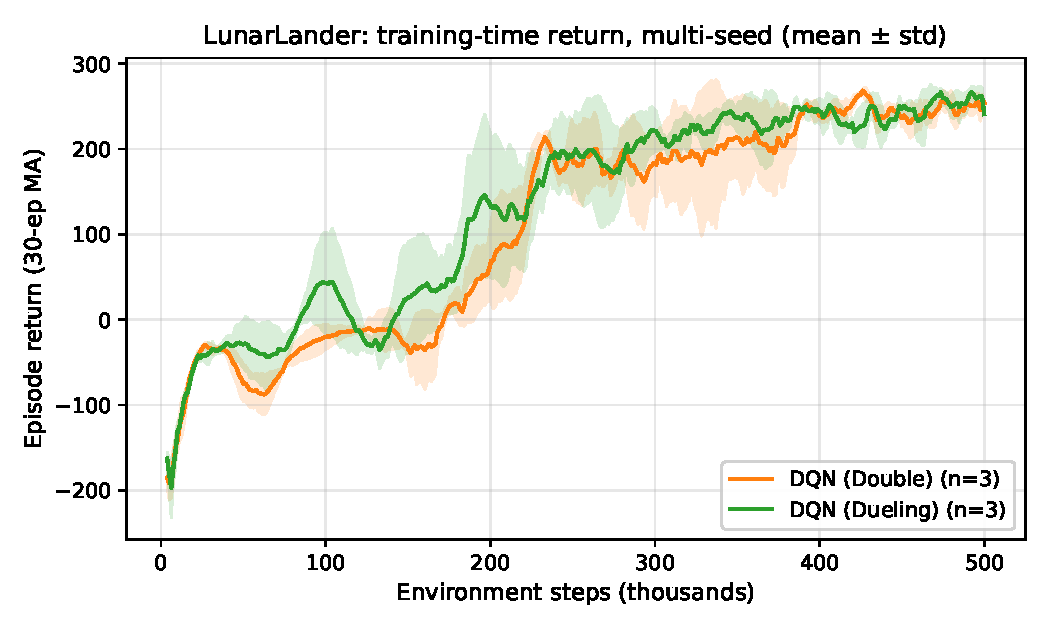
\includegraphics[width=0.42\linewidth]{figures/lander_multiseed.pdf}
\caption{LunarLander multi-seed curves (3 seeds, $\pm 1$ std band).}
\label{fig:lander_multiseed}
\end{figure}

\paragraph{Limitations.} Pong is one of the easier Atari games; harder-exploration improvements (e.g., Prioritized Experience Replay,
distributional RL) do not show their full benefit. Our Pong runs use
2\,M (seed~42) or 1.5\,M (seeds 0, 7) env steps -- well short of the
$\sim\!50$\,M-frame budget in \citet{mnih2015human} -- so final scores
are mid-curve, not asymptotic. Hyperparameter sensitivity was tested
only on LunarLander DQN.

\paragraph{Reflection and tools.} Three findings updated our prior on
deep RL. \emph{(i)~Hyperparameter dominates algorithm} -- the
factor-of-10 LR sweep moved the LunarLander score by more than the
Vanilla\,$\to$\,Double DQN change; algorithmic comparison without
hyperparameter control is unreliable~\citep{henderson2018deep}.
\emph{(ii)~Single-seed plots lie} -- the multi-seed analysis forced us to
retract the seed=42 ``Vanilla overtakes Double'' finding; the $\sigma$
gap between Dueling (0.91) and Vanilla (9.6) is invisible at $n=1$.
\emph{(iii)~Theory shows up in the data} -- the $\overline{Q}$ curve
(Fig.~\ref{fig:pong_q}) animates Thrun's 1993 overestimation argument on
our own training run. We also became viscerally aware of the cost:
$\sim\!13.5$\,M Pong env-steps were spent on the multi-seed table alone.
\emph{Tools:} An AI coding assistant helped with code scaffolding and
prose polishing; all research design, hyperparameter choices, and
interpretation are the student's. SB3~\citep{raffin2021stable},
Gymnasium~\citep{towers2024gymnasium}, and ALE~\citep{bellemare2013arcade}
are used as cited.

% ----------------------------------------------------------------------------
{\footnotesize
\setlength{\bibsep}{0pt plus 0.1ex}
\renewcommand{\baselinestretch}{0.95}\selectfont
\begin{multicols}{2}
\bibliography{references}
\end{multicols}
}

% ----------------------------------------------------------------------------
\clearpage
\appendix
\section*{Appendix: Source code listings}
\addcontentsline{toc}{section}{Appendix: Source code listings}

The following Python modules implement the full project. They are organized
to mirror the methods section: \texttt{wrappers.py} handles Atari
preprocessing; \texttt{replay\_buffer.py} the experience replay;
\texttt{networks.py} the CNN/MLP/dueling architectures; \texttt{dqn\_agent.py}
the DQN training step (Vanilla / Double / Dueling); \texttt{train\_dqn.py}
the training loop; \texttt{train\_ppo.py} the PPO entry point (using SB3);
\texttt{evaluate.py} / \texttt{evaluate\_ppo.py} the 100-episode greedy
evaluation; \texttt{evaluate\_checkpoints.py} the per-checkpoint eval used
for the learning curves in Figs.~\ref{fig:pong_curves}(b) and
\ref{fig:lander_curves}(b); \texttt{clean\_history.py} de-duplicates
crash-resumed history files; and \texttt{plot\_results.py} and
\texttt{make\_tables.py} produce all figures and tables in the body.
Total $\approx 1\,500$ lines.

\lstset{style=py}

\subsection*{\texttt{wrappers.py} -- Atari preprocessing}
\lstinputlisting[language=Python]{code_listings/wrappers.py}

\subsection*{\texttt{replay\_buffer.py} -- Uniform experience replay}
\lstinputlisting[language=Python]{code_listings/replay_buffer.py}

\subsection*{\texttt{networks.py} -- Q-network architectures}
\lstinputlisting[language=Python]{code_listings/networks.py}

\subsection*{\texttt{dqn\_agent.py} -- DQN agent (3 variants)}
\lstinputlisting[language=Python]{code_listings/dqn_agent.py}

\subsection*{\texttt{train\_dqn.py} -- DQN training loop}
\lstinputlisting[language=Python]{code_listings/train_dqn.py}

\subsection*{\texttt{train\_ppo.py} -- PPO training (SB3)}
\lstinputlisting[language=Python]{code_listings/train_ppo.py}

\subsection*{\texttt{evaluate.py} -- DQN final 100-ep evaluation}
\lstinputlisting[language=Python]{code_listings/evaluate.py}

\subsection*{\texttt{evaluate\_ppo.py} -- PPO final evaluation}
\lstinputlisting[language=Python]{code_listings/evaluate_ppo.py}

\subsection*{\texttt{evaluate\_checkpoints.py} -- Per-checkpoint eval curves}
\lstinputlisting[language=Python]{code_listings/evaluate_checkpoints.py}

\subsection*{\texttt{clean\_history.py} -- De-duplicate crash-resumed history}
\lstinputlisting[language=Python]{code_listings/clean_history.py}

\subsection*{\texttt{plot\_results.py} -- Learning curves}
\lstinputlisting[language=Python]{code_listings/plot_results.py}

\subsection*{\texttt{make\_tables.py} -- Result tables}
\lstinputlisting[language=Python]{code_listings/make_tables.py}

\end{document}
